\chapter{Commande temps discret}
Afin d'implémenter la commande, nous avons dans un premier temps évaluer les contraintes lié au support d'implémentation et dans un second temps nous allons adapter la commande de façon à ce qu'elle soit implémentable sur le micro-contrôleur. Ensuite, nous évaluerons cette transformation. Voici, ci-dessous figure \ref{fig:GeneralSCHEMA}, le schéma général des différents éléments.	
\begin{figure}[!ht]
\centering 
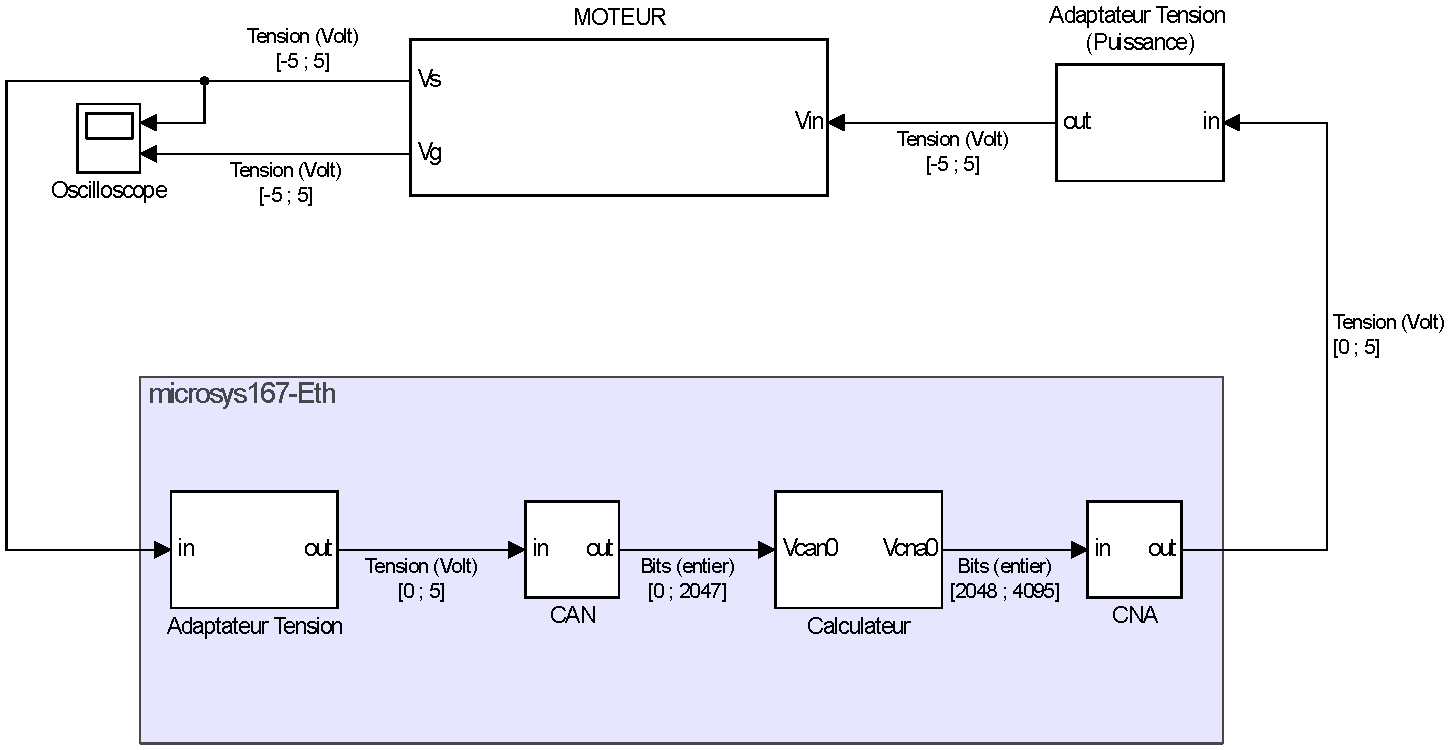
\includegraphics[width=.7\textwidth]{./V/images/schemaMO_MICRO.pdf}
\caption{\label{fig:GeneralSCHEMA}Schéma des différents composants du montage.}
\end{figure}
On remarque qu'il y a 4 composants et le détail, non exhaustif, des éléments utiles de la carte \emph{microsys167-Eth}.
Le bloc nommé moteur correspond au banc moteur présent en salle de TP. Le bloc adaptateur de tension (Puissance) est la carte qui permet de passer de la tension de commande ($0$ à $5$ Volt) vers une tension adaptée au moteur ($-5$ à $5$ Volt).
\section{Contraintes hardware} 
Nous allons, dans cette partie, nous consacrer à une étude des contraintes matérielles. Dans un premier temps nous verrons quels sont les spécificités du micro-contrôleur. Puis, nous verrons les convertisseurs analogique/numérique et numérique/analogique et nous conclurons sur le choix du micro-contrôleur. 
	\subsection{Micro-contrôleur C167}
		%(ordo,taches,validation TR,temps calcul, fréquence fonctionnement)
Pour ce projet, nous disposons d'un micro-contrôleur \emph{C167} fabriqué par Siemens. Il est dans une carte \emph{microsys167-Eth} qui lui  ajoute des interfaces, des fonctionnalités et de la mémoire. La carte cadence le micro-contrôleur à $20\text{ }MHz$, ajoute un $1\text{ }Mo$ de RAM et $512\text{ } Ko$ de Flash-EPROM. Nous disposons aussi d'adaptateurs de tension ($\left[-5;5\right]$ Volt vers $\left[0;5\right]$ Volt). Le \emph{C167} offre différentes fonctionnalités, dont les interruptions matérielles, les taches, les timers périodiques et un débogueur. Nous avons également des outils de développement permettant depuis un ordinateur, de créer un programme en \emph{C}, le compiler pour le \emph{C167}, l'envoyer sur celui-ci et si besoin de le déboguer et récupérer des valeurs sur un terminal. La fréquence de fonctionnement du \emph{C167} est de $20 $ MHz et un cycle instruction faut 4 cycle CPU, donc la fréquence d'instruction est de $5 $ MHz.
Le \emph{C167} a également des entrées et des sorties numériques et analogiques. Nous allons maintenant vous parlez des problématiques de conversions.
	\subsection{CAN / CNA}
%		(protocole correction, temps conversion, échantillonnage bits )	

%%%% CAN			
Nous allons détailler deux types de conversions nécessaires à ce projet. \\
\hspace{3mm} \textbf{CAN :} (Conversion Analogique Numérique.) Durant cette opération, le convertisseur échantillonne grâce à un bloqueur (discrétisation temporelle) puis quantifie (discrétisation de l'amplitude) le signal analogique. Il restitue un signal numérique après un temps de conversion $t_{CAN}$. Nous avons besoin de ce type de convertisseur pour la lecture des entrées dans notre cas, $V_{D}$. La qualité de notre conversion dépend de plusieurs éléments : 
\begin{itemize}
\item Le nombre de bits de sortie (la sortie ne pouvant prendre que $2^{\text{nbrBit}}$ valeurs différentes). Nous avons des CAN 11 bits.
\item La fréquence de conversion du signal analogique $f_{e}$ par rapport à la fréquence utile maximale du signal a convertir $f_{max}$. Le théorème de Shannon préconise d'avoir au moins le rapport de l'équation \ref{equ:Fshannon}, en pratique nous respecterons le rapport de l'équation \ref{equ:Freel}. Cela évite le repliement.
\begin{eqnarray}
\label{equ:Fshannon} f_e &>& 2*f_{max}\\
\label{equ:Freel} f_e & \approx & 10*f_{max}
\end{eqnarray}
Nous avons considéré que la fréquence utile maximale de la position d'un moteur à courant continue est d'environ $f_{max} = 100Hz$. Nous avons donc prendre $f_e = 1kHz$.
\item La conversion doit être linéaire. En effet, il existe différentes erreurs possibles. Il peut y avoir un offset, une erreur de gainn une non-linéarité intégrale ou différentielle (voir figure \ref{fig:errCAN}).
\end{itemize}
\begin{figure}[!ht]
\centering 
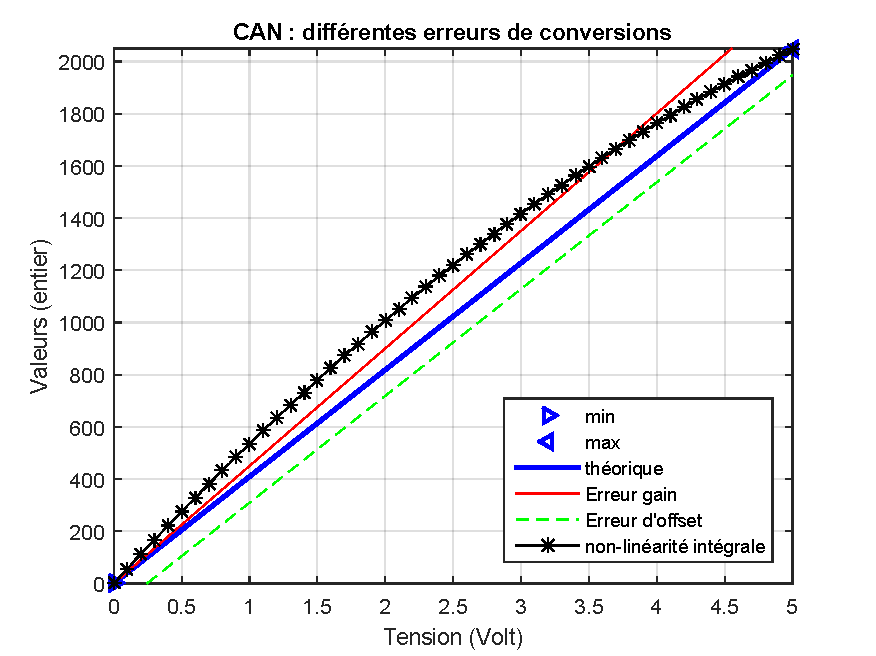
\includegraphics[width=.6\textwidth]{./V/images/CAN.pdf}
\caption{\label{fig:errCAN}Erreurs sur le CAN}
\end{figure}

%%%% CNA 
\hspace{3mm} \textbf{CNA :} (Conversion Numérique Analogique.) Ici, le convertisseur transforme le signal numérique en un signal analogique après un temps de conversion $t_{CNA}$. Nous avons besoin de ce type de convertisseur pour la génération de la sortie dans notre cas, $V_{s}$. La qualité de notre conversion dépend de plusieurs éléments similaires au CAN. L'entrée du CNA est un entier codé sur 12 bits et il génère une tension comprise entre $-5$ et $5$ Volts. 


Par manque de temps, nous n'avons pas eu le temps mettre en place un protocole complet d'étude des erreurs de conversions, nous avons uniquement vérifié que les valeurs mesurées et générées correspondent à celles désirées. Nous avons fait ceci pour quelques valeurs (min, max et milieu).

Un protocole de test complet aurait été :\\
\begin{itemize}
\item Pour le CAN : 
	\begin{itemize}
		\item Générer, à partir d'un générateur de basse tension, un signal triangle de $0$ à $5$ Volt de fréquence faible.
		\item Lire toutes les valeurs et les faire afficher sur un terminal par le micro-contrôleur.
		\item Les comparer (à l'aide d'un tableur ou de Matlab) et vérifier la linéarité de la conversion.
		\item À partir des ces résultats, créer une fonction qui corrige les erreurs, si possible.
	\end{itemize}

\item Pour le CNA :
	\begin{itemize}
		\item Générer, à partir du micro-contrôleur un signal triangle de $-5$ à $5$ Volt de fréquence faible.
		\item Récupérer les valeurs à partir d'un CAN déjà corrigé (carte d'acquisition Matlab, ou le CAN précédemment si la correction donne de très bons résultats).
		\item Les comparer (à l'aide d'un tableur ou de Matlab) et vérifier la linéarité de la conversion.
		\item À partir des ces résultats, créer une fonction qui corrige les erreurs, si possible.
	\end{itemize}
\end{itemize}
\begin{eqnarray}
T_{CAN} &=& 14*t_{cc} + 2*t_{sc} + 4*TLC \\
&=&  9,7 \mu s%\\
%T_{CNA} &=& %% TODO %%%%%%%%%%%%%%%%%%%%%%%%%%%%%%%%%%%%%%%%%%%%% /!\  %%%%%%%%%%%%%%%%%%%%%%%%%%%%%%%%%%%
\end{eqnarray}
%%%%%%%%%%%%%%%%%%%%%%%%%%%%%%%%%%%%%%%%%%%%% /!\  %%%%%%%%%%%%%%%%%%%%%%%%%%%%%%%%%%%
%%%%%%%%%%%%%%%%%%%%%%%%%%%%%%%%%%%%%%%%%%%%% /!\  %%%%%%%%%%%%%%%%%%%%%%%%%%%%%%%%%%%
%%%%%%%%%%%%%%%%%%%%%%%%%%%%%%%%%%%%%%%%%%%%% /!\  %%%%%%%%%%%%%%%%%%%%%%%%%%%%%%%%%%%\\
%%%%%%%%%%%%%%%%%%%%%%%%%%%%%%%%%%%%%%%%%%%%% /!\  %%%%%%%%%%%%%%%%%%%%%%%%%%%%%%%%%%%
	\subsection{Conclusion}
	  	(contraintes tempo, squelette code correcteur)
	  	
	  	
	  	

\section{Discrétisation de la commande}
	\subsection{Fonctions de transferts}
		 (observateur + retour état = 2 ft)
	\subsection{Transformée en z}